\documentclass{article}
\usepackage[utf8]{inputenc}
\usepackage{enumitem}
\usepackage{hyperref}
\usepackage{wrapfig}
\usepackage{graphicx}
\graphicspath{ {images/} }

\hypersetup{
    colorlinks=true,
    linkcolor=blue,
    filecolor=magenta,
    urlcolor=cyan,
    citecolor=black,
}

\title{
MIDA
\\
User Testing Guide
\\
\textit{Multi-Modality} vs \textit{AI-Assisted}
\\
First Comparison
}

\author{
Francisco Maria Calisto\\
\texttt{francisco.calisto@tecnico.ulisboa.pt}
}

\date{07/03/2019}

\begin{document}

\maketitle

\textbf{Prototype:} \hyperlink{https://github.com/mida-project/prototype-multi-modality-assistant}{prototype-multi-modality-assistant} \hfill \textbf{Version:} \hyperlink{https://github.com/mida-project/prototype-multi-modality-assistant/tree/9a912aea8d156f53e846b15bb29a09fc046bd731}{v1.0.1-alpha}

\textbf{Milestone:} \hyperlink{https://github.com/mida-project/prototype-multi-modality-assistant/milestone/1}{1.0.1-alpha} \hfill \textbf{Release:} \hyperlink{https://github.com/mida-project/prototype-multi-modality-assistant/releases/tag/v1.0.1-alpha}{v1.0.1-alpha}

\hfill

\textbf{DICOM:} \hyperlink{https://github.com/MIMBCD-UI/dicom-server}{dicom-server}

\textbf{Commit:} \hyperlink{https://github.com/MIMBCD-UI/dicom-server/tree/80191e9941c24043c7f612b2dadcd415c060bf96}{80191e9941c24043c7f612b2dadcd415c060bf96}

\hfill

\textbf{Deployment Environment:} Localhost \hfill \textbf{Deployment Server:} Localhost

\textbf{Link:} \hyperlink{http://www.breastscreening.io/dashboard/}{breastscreening.io/dashboard}

\hfill

\textbf{Main Server:} \hyperlink{http://localhost:8486/src/public/index.html}{Localhost} \hfill \textbf{Port:} 8486

\textbf{Private IP:} \hyperlink{http://localhost:8486/src/public/index.html}{localhost} \hfill \textbf{Public IP:} \hyperlink{http://localhost:8486/src/public/index.html}{localhost}

\textbf{Private Domain:} \hyperlink{http://localhost:8486/src/public/index.html}{localhost}

\hfill

\textbf{DICOM Server:} \hyperlink{http://localhost:8448/app/explorer.html}{Localhost} \hfill \textbf{Port:} 8448

\textbf{Private IP:} \hyperlink{http://localhost:8448/app/explorer.html}{localhost} \hfill \textbf{Public IP:} \hyperlink{http://localhost:8448/app/explorer.html}{localhost}

\textbf{Private Domain:} \hyperlink{http://localhost:8448/app/explorer.html}{localhost} \hfill \textbf{From:} 8448

\clearpage

%%%%%%%%%%%%%%%%%%%%%%%%%%%%%%%%%%%%%%%%%%%%%%%%%%%
%                                                 %
%                     SECTION                     %
%                                                 %
%%%%%%%%%%%%%%%%%%%%%%%%%%%%%%%%%%%%%%%%%%%%%%%%%%%

\section{Introduction}
\label{sec:sec001}

This document aims to describe the protocol performing a set of tests in the scope of \hyperlink{https://github.com/mida-project/prototype-multi-modality-assistant/releases/tag/v1.0.1-alpha}{v1.0.1-alpha} version from the \hyperlink{https://github.com/mida-project/prototype-multi-modality-assistant}{prototype-multi-modality-assistant} repository of the \hyperlink{https://mida-project.github.io/}{MIDA} project using traditional devices (mouse and keyboard). The goal of the test is to understand the user, performance, efficiency and efficacy metrics in a context of an Artificial Intelligence (AI) diagnosis \cite{fan2018investigating}, hereby denominated as \textbf{Assistant}. The sessions will be recorded via video on the computer and using a record, heat-map and triggered event tools. It is guaranteed the confidentiality of the recordings, which will be used only for academic purposes.

Dividing the activity session into four distinct phases per each three activities representing three different scenarios (Single-Modality vs Multi-Modality vs Assistant). The first three phases took place on an \hyperlink{https://github.com/MIMBCD-UI/testing-guide-breast/tree/master/samples/test_4}{early} stage of the \textit{User Tests} while we were focus to publish on the \hyperlink{https://chi2019.acm.org/}{CHI'19 Conference}. The fourth phase will cover the hereby \textit{User Testing Guide}. Still, we will describe as follows the overall of the four phases to give higher context.

Each scenario will have three patients. In both two scenarios, by supporting our traditional devices, the interaction is made with mouse and keyboard. The first phase, is the \hyperlink{https://docs.google.com/forms/d/1cGmaCGZjeLJhUl_My2wxJ7gcpm7vQRxYhds6Ys0NoSc/edit?usp=sharing}{demographic questionnaire}, where we characterise the Radiologist profile. The second phase is the act of classifying those patients. Radiologists will classify each patient by using the \hyperlink{https://en.wikipedia.org/wiki/BI-RADS}{BIRADS}~\cite{balleyguier2007birads}. On the third phase, we will do several small questionnaires at the end of each scenario using \hyperlink{https://en.wikipedia.org/wiki/NASA-TLX}{NASA-TLX}~\cite{ramkumar2017using}, \hyperlink{https://en.wikipedia.org/wiki/System_usability_scale}{System Usability Scale (SUS)}~\cite{orfanou2015perceived} and measuring the \hyperlink{https://en.wikipedia.org/wiki/BI-RADS}{BIRADS}~\cite{balleyguier2007birads}. Finally, the fourth phase, and most importantly to this \textit{User Testing Guide}, we will provide to the clinicians the \textbf{Assistant} suggestion for the \hyperlink{https://en.wikipedia.org/wiki/BI-RADS}{BIRADS}~\cite{balleyguier2007birads} results and justification of the prognostic. For the user tests we used a three distinct prototype repositories \hyperlink{https://github.com/MIMBCD-UI/prototype-multi-single}{prototype-multi-single}, \hyperlink{https://github.com/MIMBCD-UI/prototype-multi-modality}{prototype-multi-modality} and \hyperlink{https://github.com/mida-project/prototype-multi-modality-assistant}{prototype-multi-modality-assistant}, the three are similar mirrors of the \hyperlink{https://github.com/MIMBCD-UI/prototype-breast-cancer}{prototype-breast-cancer} with minor changes.
%%%%%%%%%%%%%%%%%%%%%%%%%%%%%%%%%%%%%%%%%%%%%%%%%%%
%                                                 %
%                     SECTION                     %
%                                                 %
%%%%%%%%%%%%%%%%%%%%%%%%%%%%%%%%%%%%%%%%%%%%%%%%%%%

\section{Material}
\label{sec:sec002}

For the material and apparatus, it is essential to capture the session apprehending the user interactions. In our case, we will record this interaction by using the \hyperlink{https://support.apple.com/quicktime}{QuickTime Player Version 10.4 (928.5.1)} to obtain all interactions. We will pair this video tool with a user watch tool called \hyperlink{https://www.hotjar.com/}{Hotjar}. This tool serves the purpose of using several logs of the interaction and gives us visualisation over it. Both instruments will help us to capture where are users interacting. By looking at the test participant's reactions, we find a lot of information regarding the prototype design.

\clearpage

The tools that we choose for the material and apparatus of this User Testing Guide are low-cost and easy to use. Our equipment is a cost-effective and, by using our laboratory materials, bringing it to the radiology room, we enable to capture not only what the user is doing on the screen, but on the body language supported by the interviews and observation.

\hfill

The material used in the test sessions for the user interface consists of:

\hfill

\begin{itemize}
  \item MacBook Pro: it will allow the user to interact with the keyboard and a wireless mouse;
  \item Wireless Mouse: it will allow the user to interact with a mouse and will complement the keyboard;
\end{itemize}

\hfill

%%%%%%%%%%%%%%%%%%%%%%%%%%%%%%%%%%%%%%%%%%%%%%%%%%%
%                                                 %
%                     SECTION                     %
%                                                 %
%%%%%%%%%%%%%%%%%%%%%%%%%%%%%%%%%%%%%%%%%%%%%%%%%%%

\subsection{Technical Details}

To produce this traditional environment, and since we can simulate with a laptop, the mouse and keyboard interaction, we are using a Microsoft Mobile Mouse 4000 together with the \hyperlink{https://www.apple.com/shop/buy-mac/macbook-pro}{MacBook Pro} (Retina, 13-inch, Early 2015) with a standard integrated keyboard on the laptop.

%%%%%%%%%%%%%%%%%%%%%%%%%%%%%%%%%%%%%%%%%%%%%%%%%%%
%                                                 %
%                     SECTION                     %
%                                                 %
%%%%%%%%%%%%%%%%%%%%%%%%%%%%%%%%%%%%%%%%%%%%%%%%%%%

\subsection{Software}

To track our user interactions across our system, we are using \hyperlink{https://www.hotjar.com/}{Hotjar}. This tool is an analytic package allowing us to follow our users remotely. It also provides two critical pieces of functionality, among others, that can aid in remote user testing. First of all, the heatmaps allow us to see where users are clicking, tapping and scrolling on our system. Second, it records a video playback of the entire user session. The tool shows evidence of being useful for our studies while we successfully used it in the past.

To record the task activities and the interview, we used \hyperlink{https://support.apple.com/downloads/quicktime}{QuickTime}~\cite{rowell2006internet}. The \hyperlink{https://support.apple.com/downloads/quicktime}{QuickTime} (\hyperlink{https://www.apple.com/}{Apple Computer}) tool is available for \hyperlink{https://www.apple.com/shop/buy-mac/macbook-pro}{MacBook Pro} to movie, audio and screen recording. Despite of have an overall of features, we just used it for our user's screen recording. It provides this functionalities at minimum requirements and compatible to our apparatus.

\clearpage
%%%%%%%%%%%%%%%%%%%%%%%%%%%%%%%%%%%%%%%%%%%%%%%%%%%
%                                                 %
%                     SECTION                     %
%                                                 %
%%%%%%%%%%%%%%%%%%%%%%%%%%%%%%%%%%%%%%%%%%%%%%%%%%%

\section{Description}
\label{sec:sec003}

To verify our work, we identified measurable and explicit targets. By having several goals, including that a value percentage of the users should be able to operate the tasks without the need of help. On the same rate value, the user should be able to start and complete the medical diagnosis tasks over the system with little errors or mitigating those errors. Measuring the expected number of errors with a relation between our laboratory pilot tests. On the laboratory pilot tests we aim to test our prototypes with researchers. The Researchers are in the context of the system and know well the functionalities so that we need to expect a percentage value over their results compared to clinicians and not the same benefits. Last but not least, both users (researchers and clinicians) should be able to understand in a similar time amount the meaning of all visible controls. By the similar amount of time, it is expected to have a variance of the percentage value between researchers and clinicians of the same value percentage of the early goals described in this paragraph.

We tested each objective in early laboratory and field tests so that we could take the appropriate corrective actions. Also, we expect to run early field tests with researchers and clinicians to highlight issues that we overlooked and ignored during the prototyping phase. To support interaction use by the clinicians, we will try to emphasise several key factors on our user tests. The tasks must be simple, low intrusive, support for natural interaction and the system must always give visibility and the task current-state.

\clearpage

%%%%%%%%%%%%%%%%%%%%%%%%%%%%%%%%%%%%%%%%%%%%%%%%%%%
%                                                 %
%                     SECTION                     %
%                                                 %
%%%%%%%%%%%%%%%%%%%%%%%%%%%%%%%%%%%%%%%%%%%%%%%%%%%

\subsection{Devices}

Traditional interaction remains the most common way to interact with user interfaces in a clinical environment. Unfortunately, most of this interaction is made by low profile equipment that makes users produce more errors and take more time interacting with those user interfaces.

On Figure \ref{fig:patient_list} the user can select the list of patients. The list has a table with several patient information. The first column is the \textit{Patient ID}; we used it as an identifier of the patient. That way we can have anonymised information with no reference to the patient name. The second column is the \textit{Study Date}, the third column is the \textit{Modality} of the used \textbf{DICOM} image, the fourth column is the \textit{Study Description} of the used study and the last column is the number of \textit{Images}.

%%%%%%%%%%%%%%%%%%%%%%%%%%%%%%%%%%%%%%%%%%%%%%%%%%%

\hfill

\begin{figure}[h]
\centering
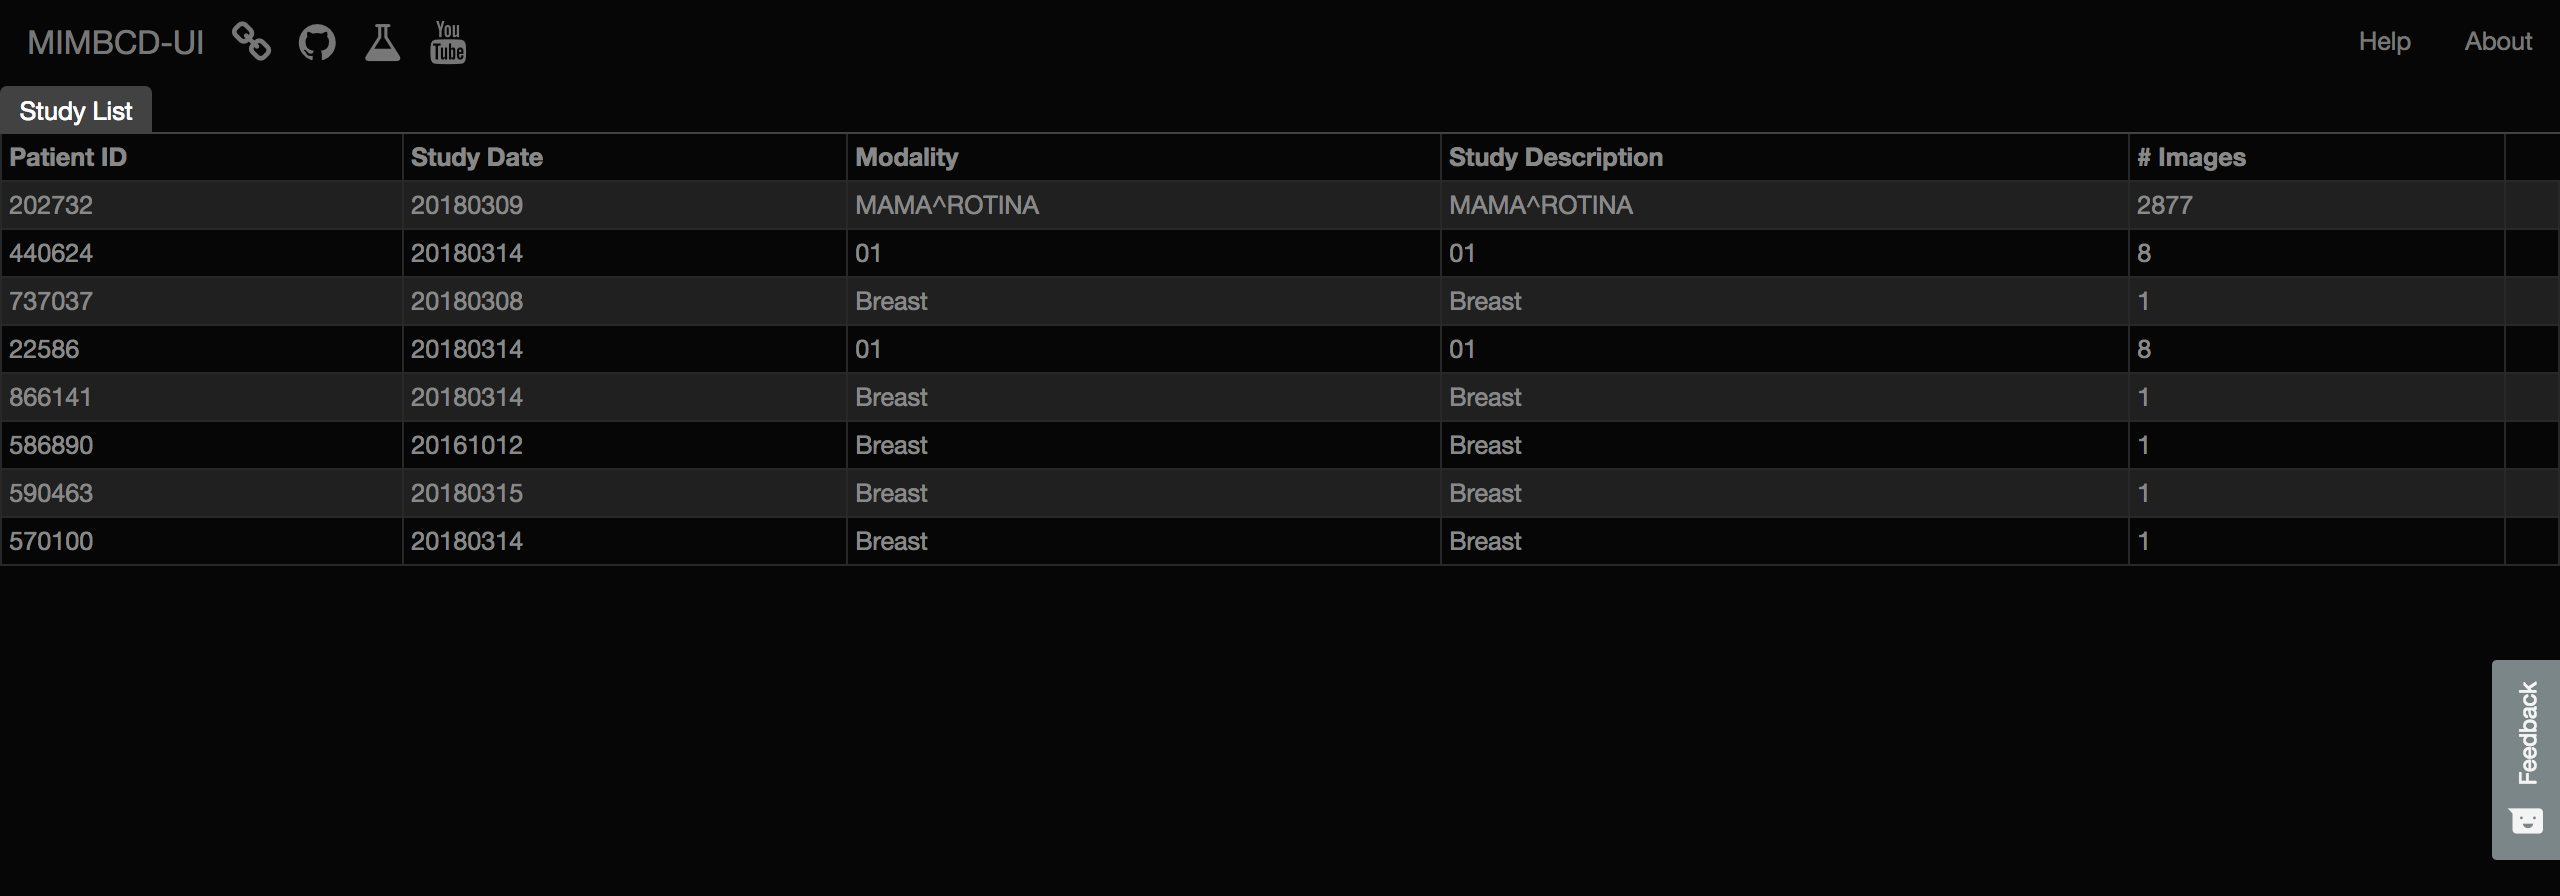
\includegraphics[width=\textwidth]{patient_list}
\caption{List of Patients.}
\label{fig:patient_list}
\end{figure}

\hfill

%%%%%%%%%%%%%%%%%%%%%%%%%%%%%%%%%%%%%%%%%%%%%%%%%%%

As we can see in Figure \ref{fig:image_viewer}, it shows the first task in our User Interface (UI), where the patient's breasts are on a small left column. The options are in a short row near of the viewport and described below. We also have the tabs where the user can change the patient. The centre viewport shows the \textbf{DICOM} image, and it can be configured to display a number up to four \textbf{DICOM} images at the same time. The viewport has some text information on it (yellow) with the details of the metadata. Nevertheless, the \textbf{Assistant} suggestions are shown on the top-right corner of the system.

\clearpage

%%%%%%%%%%%%%%%%%%%%%%%%%%%%%%%%%%%%%%%%%%%%%%%%%%%

\hfill

\begin{figure}[h]
\centering
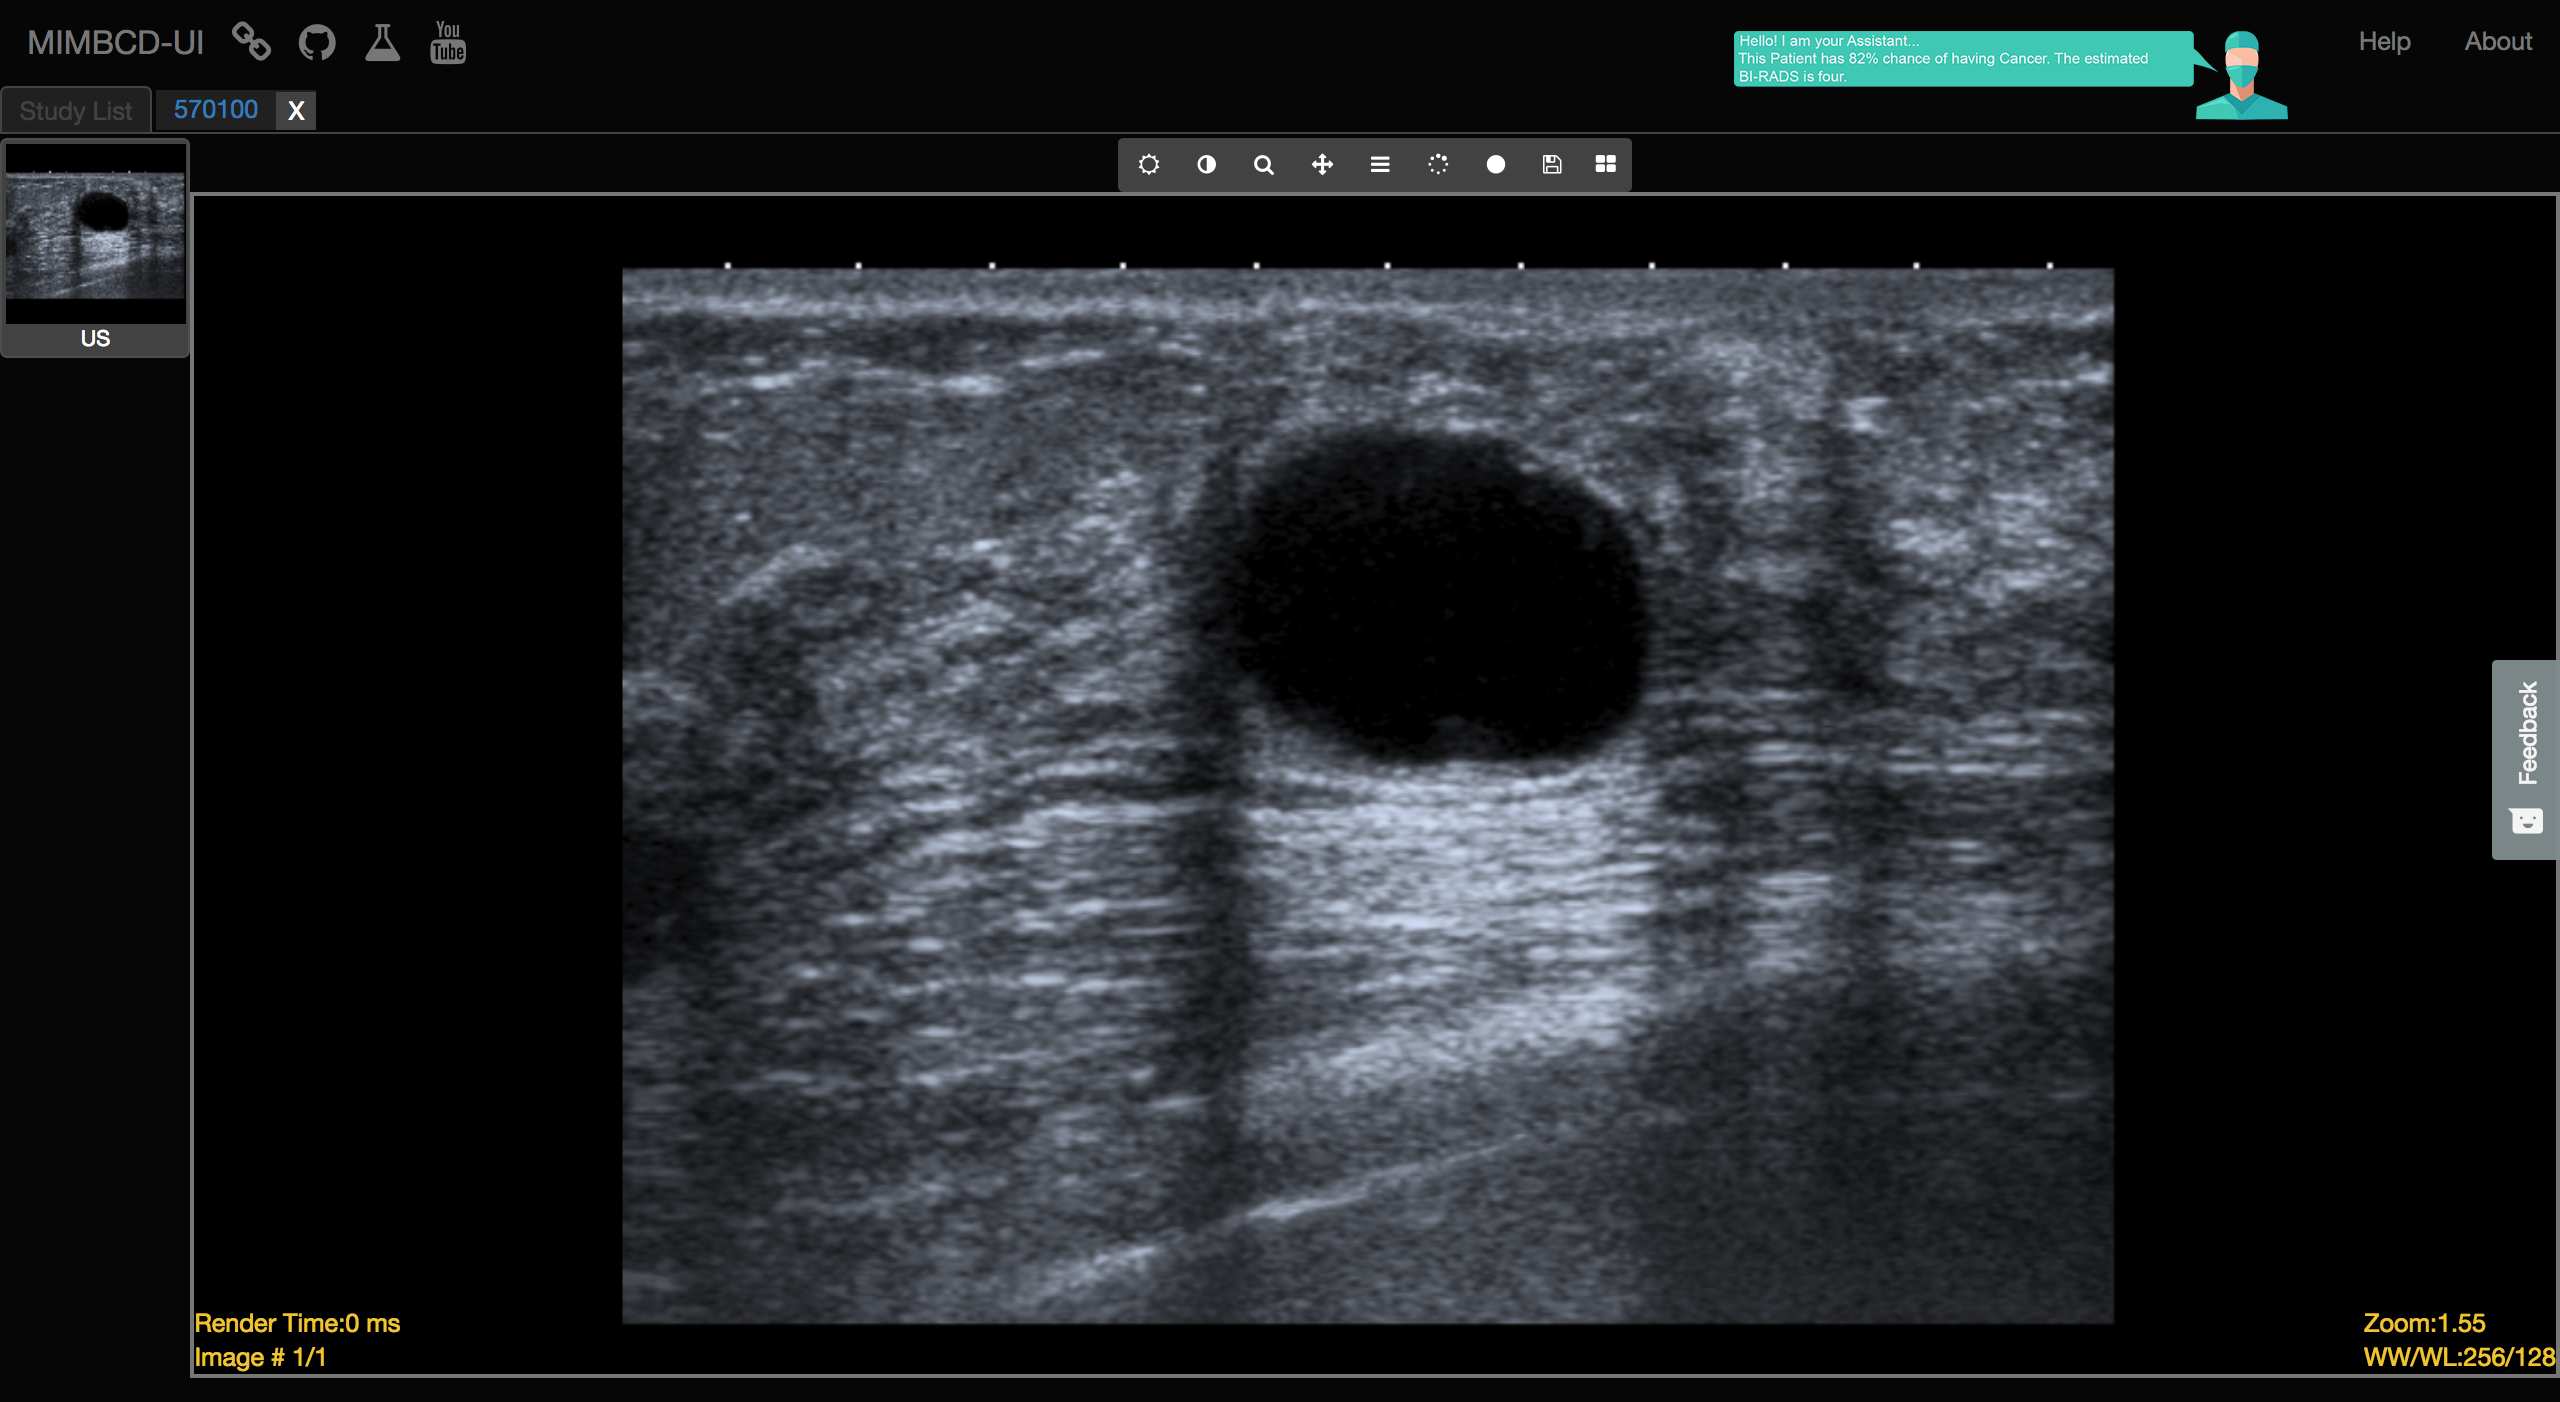
\includegraphics[width=\textwidth]{image_viewer}
\caption{Viewer of the \textbf{DICOM} images.}
\label{fig:image_viewer}
\end{figure}

\hfill

%%%%%%%%%%%%%%%%%%%%%%%%%%%%%%%%%%%%%%%%%%%%%%%%%%%

Manual annotation~\citation{cao2015collaborative} is adopted by us thanks to Freehand ROI and Probe annotation features, both from \hyperlink{https://cornerstonejs.org/}{CornerstoneJS}. According to the \hyperlink{https://cornerstonejs.org/}{CornerstoneJS} Library, the user can create an annotation by setting up consecutive landmarks around a Region of Interest (ROI). The markers finish a lesion annotation when it interconnects the historical. Additional features available in our User Interface (UI) includes on-demand increment of the number of landmarks, and throw transformations of the shape of an annotation.

\clearpage

%%%%%%%%%%%%%%%%%%%%%%%%%%%%%%%%%%%%%%%%%%%%%%%%%%%
%                                                 %
%                     SECTION                     %
%                                                 %
%%%%%%%%%%%%%%%%%%%%%%%%%%%%%%%%%%%%%%%%%%%%%%%%%%%

\subsection{User Interactions}

The systems have several buttons (Figure \ref{fig:toolbar}) that allows the user to interact or access to a set of user interface features. Each item of the following list represents each metaphoric icon of Figure \ref{fig:toolbar}.

%%%%%%%%%%%%%%%%%%%%%%%%%%%%%%%%%%%%%%%%%%%%%%%%%%%

\hfill

\begin{figure}[h]
\centering

\includegraphics[width=\textwidth]{toolbar}
\caption{Toolbar of the System available features.}
\label{fig:toolbar}
\end{figure}

\hfill

%%%%%%%%%%%%%%%%%%%%%%%%%%%%%%%%%%%%%%%%%%%%%%%%%%%

\hfill

The buttons are (from left to right of Figure \ref{fig:toolbar}) as follows:

\hfill

\begin{itemize}
\item WW/WC
\item Invert
\item Zoom
\item Pan
\item Stack Scroll
\item Freehand
\item Probe
\item Save
\item Window Controller
\end{itemize}

\hfill

\clearpage

%%%%%%%%%%%%%%%%%%%%%%%%%%%%%%%%%%%%%%%%%%%%%%%%%%%
%                                                 %
%                     SECTION                     %
%                                                 %
%%%%%%%%%%%%%%%%%%%%%%%%%%%%%%%%%%%%%%%%%%%%%%%%%%%

\subsection{Evaluation}

Introduction of AI \textbf{Assistant} agents are significant factors which can naturally affect the performance of a medical workflow. While some prior studies \cite{Calisto:2017:TTM:3132272.3134111, calisto2017mimbcdui} have investigated the functionality of healthcare systems, the \textit{AI-Assisted} acceptability has mostly been overlooked in the existing Health Informatics (HI) literature regarding a Human-Computer Interaction (HCI).

The following Table \ref{table:usability_evaluation_questions} is presenting seven evaluation questions to have in mind during evaluation. The purpose of this questions is to facilitate systematic user studies regarding our novel \textbf{Assistant} in a clinical environment and support user stimulation for the introduction of \textit{AI-Assisted} methods. The proposed issues involve various aspects of workflow combined with either need for satisfaction or division of attention.

\hfill

\begin{table}[h]
\centering
\begin{tabular}{l|l}
Number & Issues of Content \& Key Questions                    	 \\ \hline
1      & How would the user describe the potential adoption of   \\
       & \textit{AI-Assisted} methods on the Health Institution? \\ \hline
2      & What are the user oppositions for \textit{AI-Assisted}	 \\
       & methods?                                                \\ \hline
3      & What examples of \textit{AI-Assisted} methods does the  \\
       & user know regarding the Health Institution?             \\ \hline
4      & What are the obstacles of the user's Health             \\
       & Institution?                                            \\ \hline
5      & What is more important for the \textit{AI-Assisted}     \\
       & information, the BIRADS or Pathology?                   \\ \hline
6      & Is it important for the user to have the feature of		 \\
       & Approve, Reject and Justify options?                    \\ \hline
7      & For the user's opinion, what are the aspects that       \\
       & influence the decision?                                 \\ \hline

\end{tabular}
\caption{Usability Evaluation Questions}
\label{table:usability_evaluation_questions}
\end{table}

\hfill

The influence of \textit{AI-Assisted}~\cite{goodfellow2016deep} is an important variable for our empirical analysis. In fact, the trust of the user increases when the user perceived that the \textbf{Assistant} is giving the right inputs and that there will be a consequent increase of the clinician trust in our system.

\clearpage

The first question, the \textit{How would the user describe the potential adoption of \textit{AI-Assisted} methods on the Health Institution?} question. For the second question, the \textit{What are the user oppositions for \textit{AI-Assisted} methods?} question, we aim to understand what are the user constrains regarding an AI adoption the the user's current workflow. Third, we intend to filter possible examples of the clinical applications of AI on the Health Institutions by asking \textit{What examples of \textit{AI-Assisted} methods does the user know regarding the Health Institution?} directly to the clinician. The fourth question, underlines the reasons why several obstacles are present on the Health Institution, with the question \textit{What are the obstacles of the user's Health Institution?} we can understand the challenges of achieving those issues and what are the solutions for surpass it. On the fifth question, where we ask \textit{What is more important for the \textit{AI-Assisted} information, the BIRADS or Pathology?}, we aim to understand what is more important for the user, the BIRADS or the Pathology~\cite{maicas2018pre} of the patient~\cite{elverici2015nonpalpable}. Almost last, the six question, where we ask for \textit{Is it important for the user to have the feature of \textbf{Approve}, \textbf{Reject} and \textbf{Justify} options?} is an important question to understand the feature needs and options. Last but not least, the seven question, \textit{For the user's opinion, what are the aspects that influence the decision?}, is where we will understand what is the most important information to show to the clinicians, therefore, we can more effectively and efficiently give more accurate information to the users.

To conclude this section, by doing this questions, we aim to support our user studies by giving our users, the clinicians, the opportunity of improving our empirical analysis regarding user's \textit{open answers}. However, the results should be treated with caution. Several bias exists since we are doing here an ambiguous approach.

\clearpage
%%%%%%%%%%%%%%%%%%%%%%%%%%%%%%%%%%%%%%%%%%%%%%%%%%%
%                                                 %
%                     SECTION                     %
%                                                 %
%%%%%%%%%%%%%%%%%%%%%%%%%%%%%%%%%%%%%%%%%%%%%%%%%%%

\section{Methodology}
\label{sec:sec004}

The hereby prototype used is the \hyperlink{https://github.com/mida-project/prototype-multi-modality-assistant/releases/tag/v1.0.1-alpha}{v1.0.1-alpha} version of our \hyperlink{https://github.com/mida-project/prototype-multi-modality-assistant/}{prototype-multi-modality-assistant}. The purpose of this prototype is to involve an \textit{AI-Assisted} tool (\textbf{Assistant}) for medical imaging at a breast screening diagnosis level. This \textbf{Assistant} was created with a front-end and bak-end architecture utilising common programming languages, libraries, frameworks and tools including \hyperlink{https://www.javascript.com/}{JavaScript (JS)}~\cite{flanagan2006javascript}, \hyperlink{https://nodejs.org/}{NodeJS}~\cite{wilson2018node}, \hyperlink{https://hammerjs.github.io/}{HammerJS}, \hyperlink{https://cornerstonejs.org/}{CornerstoneJS}~\cite{hostetter2018integration} and \hyperlink{https://www.orthanc-server.com/}{Orthanc}~\cite{Jodogne:ISBI2013}. For the Machine Learning (ML) and Deep Learning (DL)~\cite{ribeiro2017real, ribeiro2016real} component we will use several \hyperlink{https://www.mathworks.com/products/matlab.html}{MATLAB} technologies~\cite{vedaldi2015matconvnet}, promoting and feeding our Convolutional Neural Networks (CNN)~\cite{carneiro2015unregistered} and Deep Reenforcement Learning (DRL)~\cite{maicas2017deep} techniques. Other central component of this prototype is a web-based \hyperlink{https://www.sciencedirect.com/topics/medicine-and-dentistry/picture-archiving-and-communication-system}{PACS}~\cite{cooke2003picture} pairwise with ubicous web technologies and based on the \textbf{Open Source (OS)} \hyperlink{https://cornerstonejs.org/}{CornerstoneJS} library~\cite{feller2002understanding, hostetter2018integration}.

%%%%%%%%%%%%%%%%%%%%%%%%%%%%%%%%%%%%%%%%%%%%%%%%%%%
%                                                 %
%                     SECTION                     %
%                                                 %
%%%%%%%%%%%%%%%%%%%%%%%%%%%%%%%%%%%%%%%%%%%%%%%%%%%

\subsection{Environments}

This section describes the user environment over interaction, the so called \textbf{Radiology Room (RR)} (Figure \ref{fig:radioroom}). This guide is based on soft-copy diagnosis using computer workstations in their current reading room environment. It will be here where we take impressions regarding the efficacy of radiologists, and their recommendations based on their experience for improvements on the soft-copy reading environment. Several studies demonstrated~\cite{waite2017tired} that radiologist fatigue levels and performance are related to environmental factors such as number of false-negative and false-positives in addition to workstation enhancements. Supported by this guide, our research aims to conduct an investigation for the several environmental variables and improvements regarding the potentially enhancement that an \textit{AI-Assisted} diagnosis could take in the \textbf{RR}. We expect to analyse the needed information and best solution to improve the workstation results.

%%%%%%%%%%%%%%%%%%%%%%%%%%%%%%%%%%%%%%%%%%%%%%%%%%%

\hfill

\begin{figure}[h]
\centering
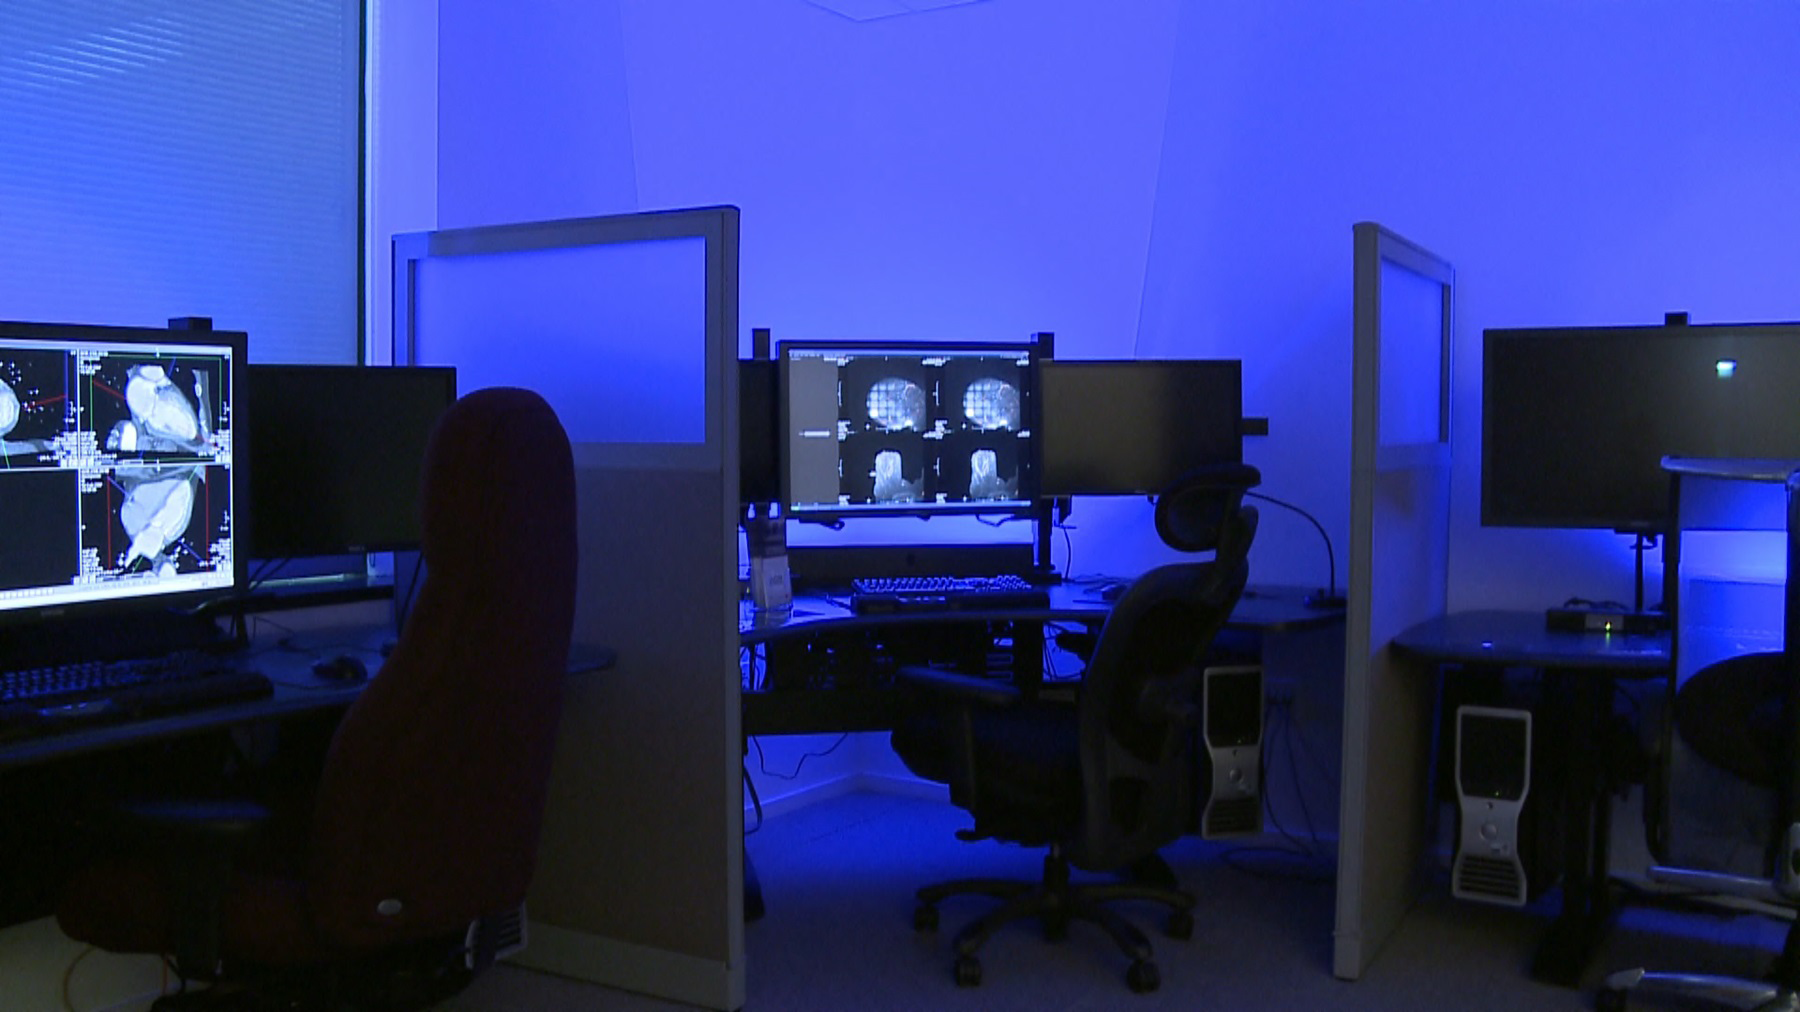
\includegraphics[width=\textwidth]{acr}
\caption{Radiology Room}
\label{fig:radioroom}
\end{figure}

\hfill

%%%%%%%%%%%%%%%%%%%%%%%%%%%%%%%%%%%%%%%%%%%%%%%%%%%

%%%%%%%%%%%%%%%%%%%%%%%%%%%%%%%%%%%%%%%%%%%%%%%%%%%
%                                                 %
%                     SECTION                     %
%                                                 %
%%%%%%%%%%%%%%%%%%%%%%%%%%%%%%%%%%%%%%%%%%%%%%%%%%%

\subsection{Case Studies}

The functionality of the prototype will be best demonstrated by a series of case studies. By describing the expected workflow and capabilities of the research study at the \textbf{RR} specific environment and changes of the workflow by using our system prototype. The study implies the evaluation of medical imaging \textit{AI-Assisted} features on several breast lesions. The primary goal of this case studies analysis is to generate a receiver operating characteristic to evaluate the performance and validation of our \textbf{Assistant}. Let us consider a list of hypothetical use cases for the research investigation that evaluates the interaction and usability performance of the \textbf{Assistant}. Therefore, the following list will show the preliminary case studies.

\hfill

List of case studies to analyse our solution prototype:

\hfill

\begin{itemize}
\item Multi-Modality \textit{AI-Assisted} of a Breast Cancer Diagnosis;
\item Priority \& Minimal Information Visualisation;
\item Performance \& Response Measurement Values Acquisition;
\item Radiologist Validation;
\end{itemize}

\hfill

%%%%%%%%%%%%%%%%%%%%%%%%%%%%%%%%%%%%%%%%%%%%%%%%%%%

We expect to demonstrate several uses through a series of case studies, including implementation of our research prototype using an \textit{AI-Assisted} technique and features for several view studies and other imaging research, as well as creation of a novel \textbf{Assistant} for the purpose. By creating a set of questions, we will try to achieve and feed this case studies. It is automatically associated with all cases. The radiologist may interact with our \textbf{Assistant} while manipulating the medical imaging and report to us difficulties and improvements. The number of questions is not restricted to the present document, since the interview will be open and suggestive~\cite{joyce2017healthcare}. There is no limit to the number of questions that can be asked per case but it should fit the amount of expected time per each.

The data will be collect from the study video and observations into a \hyperlink{https://docs.google.com/spreadsheets/d/1CoPLONnINdBWryGs7SBRuPZA-DnQ0t_yzx3u8ym0UoI/edit?usp=sharing}{spreadsheet} for further analysis. We will \hyperlink{https://github.com/mida-project/research-reports}{report} the results of this tests and conclusions. This guide and respective use cases will be iteratively improved.

\clearpage
\section{Procedures}
\label{sec:sec005}

Participants will take part in the tests at our formed institution protocols (e.g. \hyperlink{http://hff.min-saude.pt/}{Hospital Fernando Fonseca (HFF)}) with the \hyperlink{https://github.com/mida-project/prototype-multi-modality-assistant/releases/tag/v1.0.1-alpha}{v1.0.1-alpha} version of our \hyperlink{https://github.com/mida-project/prototype-multi-modality-assistant}{prototype-multi-modality-assistant} repository. The interaction with the system will be used in a typical \textbf{RR} environment. Note takers and data logger(s) will monitor the sessions for observation in the \textbf{RR}, connected by screen recording feed. The test sessions will be recorded and further analysed.

%%%%%%%%%%%%%%%%%%%%%%%%%%%%%%%%%%%%%%%%%%%%%%%%%%%
%                                                 %
%                     SECTION                     %
%                                                 %
%%%%%%%%%%%%%%%%%%%%%%%%%%%%%%%%%%%%%%%%%%%%%%%%%%%

\subsection{Briefing}

A presentation of the \textbf{Assistant} and it's use and capabilities will be made. Participants will be presented to the available interactions and will be explained how to interact with the prototype, underlining the limitations. The facilitator will brief the participants on the \textbf{Assistant} application and instruct the participant that they are evaluating the application, rather than the facilitator evaluating the participant. Participants will sign an informed consent that acknowledges: the participation is voluntary, that participation can cease at any time, and that the session will be videotaped but their privacy of identification will be granted. The facilitator will ask the participant if they have any question.

%%%%%%%%%%%%%%%%%%%%%%%%%%%%%%%%%%%%%%%%%%%%%%%%%%%

%%%%%%%%%%%%%%%%%%%%%%%%%%%%%%%%%%%%%%%%%%%%%%%%%%%
%                                                 %
%                     SECTION                     %
%                                                 %
%%%%%%%%%%%%%%%%%%%%%%%%%%%%%%%%%%%%%%%%%%%%%%%%%%%

\subsection{Post-Task Questionnaire}

Our metrics will refer the \textit{AI-Assisted} involvement against specific goals necessary to satisfy several requirements of our \textbf{Assistant}. For our \textbf{Post-Task Questionnaire} we will use \textit{Quantitative Analysis} (QtA) and \textit{Qualitative Analysis} (QlA) in response to our questions (Section \ref{sec:sec003}) to measure the acceptability of our \textbf{Assistant} each time a \textit{scenario} is completed (Section \ref{sec:sec003}). From a set of tasks (Section \ref{sec:sec006}) we aim to cover our main scenario, an \textit{AI-Assisted} that we call \textbf{Assistant}. Therefore, both QtA and QlA will allow the facilitator to quickly and easily assess the requirements of the given scenario. Our QtA and QlA requirements will have several attributes~\cite{joyce2017healthcare} that make it a good choice for our clinical participants. Those attributes are as follows.

\hfill

%%%%%%%%%%%%%%%%%%%%%%%%%%%%%%%%%%%%%%%%%%%%%%%%%%%

List of the scale attributes:

%%%%%%%%%%%%%%%%%%%%%%%%%%%%%%%%%%%%%%%%%%%%%%%%%%%

\hfill

\begin{itemize}
  \item The requirements are technology agnostic, making it flexible enough;
  \item The requirements are relatively quick and easy to answer;
  \item The requirements provide a single score on a scale that is easily understood;
  \item The requirements are nonproprietary, making it a cost effective tool;
\end{itemize}

\hfill

%%%%%%%%%%%%%%%%%%%%%%%%%%%%%%%%%%%%%%%%%%%%%%%%%%%

\clearpage

The facilitator will explain that the amount of time taken to complete the \textit{tasks} will be measured and that exploratory behaviour outside the \textit{task} flow should not occur until after task completion. At the beginning of each task, the participant will listen the \textit{task} description from the facilitator and begin the task. \textit{Time-on-Task} (ToT) measurements begins when the participant starts the \textit{task}, measured until the end of each \textit{task}.

%%%%%%%%%%%%%%%%%%%%%%%%%%%%%%%%%%%%%%%%%%%%%%%%%%%

%%%%%%%%%%%%%%%%%%%%%%%%%%%%%%%%%%%%%%%%%%%%%%%%%%%
%                                                 %
%                     SECTION                     %
%                                                 %
%%%%%%%%%%%%%%%%%%%%%%%%%%%%%%%%%%%%%%%%%%%%%%%%%%%

\subsection{Training Session}

The participant will receive and overview the test procedure. However, the user will not receive information how to annotate and interact in all degrees of freedom. With the aim of disabling users to get their work done before the test tasks. It will take advantage of a "surprise" acknowledgement.

%%%%%%%%%%%%%%%%%%%%%%%%%%%%%%%%%%%%%%%%%%%%%%%%%%%
%                                                 %
%                     SECTION                     %
%                                                 %
%%%%%%%%%%%%%%%%%%%%%%%%%%%%%%%%%%%%%%%%%%%%%%%%%%%

\subsection{Execution of Tasks}

The \textit{tasks} were derived from test scenarios developed from \textbf{Case Studies}. Due to the range and extent of functionality provided by our \textbf{Assistant}, and the short time from which each participant will be available, the \textit{tasks} are the most common and relatively complex of available functions. The \textit{tasks} are the identical for all participants of a given user role in the study.

The \textit{tasks} will be performed by several classes of radiology experience. Professionals from Radiology Seniors, Middles, Juniors and Interns will be performing these \textit{tasks}. On the \textbf{RR} the Radiologist is characterised~\cite{ehrlich2016patient, miglioretti2007radiologist} as a physician who examines and interpret Medical Imaging (MI) \cite{kobashi2017evaluation}, such as X-Rays, CT Scans or MRIs.

%%%%%%%%%%%%%%%%%%%%%%%%%%%%%%%%%%%%%%%%%%%%%%%%%%%

%%%%%%%%%%%%%%%%%%%%%%%%%%%%%%%%%%%%%%%%%%%%%%%%%%%
%                                                 %
%                     SECTION                     %
%                                                 %
%%%%%%%%%%%%%%%%%%%%%%%%%%%%%%%%%%%%%%%%%%%%%%%%%%%

\subsection{Post-Activity Questionnaire}

After completing all \textit{tasks} and scenarios, participants will be asked to complete a questionnaire to classify the \textbf{Assistant} according to various parameters regarding the several features. To measure this, we will use an open session \textit{observation} and \textit{interview}~\cite{carayon2015systematic}. We will use this techniques to identify participants' requirements during the various stages of the workflow.

%%%%%%%%%%%%%%%%%%%%%%%%%%%%%%%%%%%%%%%%%%%%%%%%%%%
\section{Tasks}
\label{sec:sec006}

During our user tests, we need to ask participants to provide a subjective assessment of their experience using our \textbf{Assistant}. There are several widely used questionnaires giving us different prons-and-cons. However, in most cases, a \hyperlink{https://www.nngroup.com/articles/keep-online-surveys-short/}{single question instrument}~\cite{sauro201210} is the right method for a quantitative usability testing. By taking less time and effort to answer, participants are pursuing to this phase after task while it is minimally disruptive.

\clearpage

%%%%%%%%%%%%%%%%%%%%%%%%%%%%%%%%%%%%%%%%%%%%%%%%%%%

\hfill

\begin{wrapfigure}{r}{0.50\textwidth}
\centering
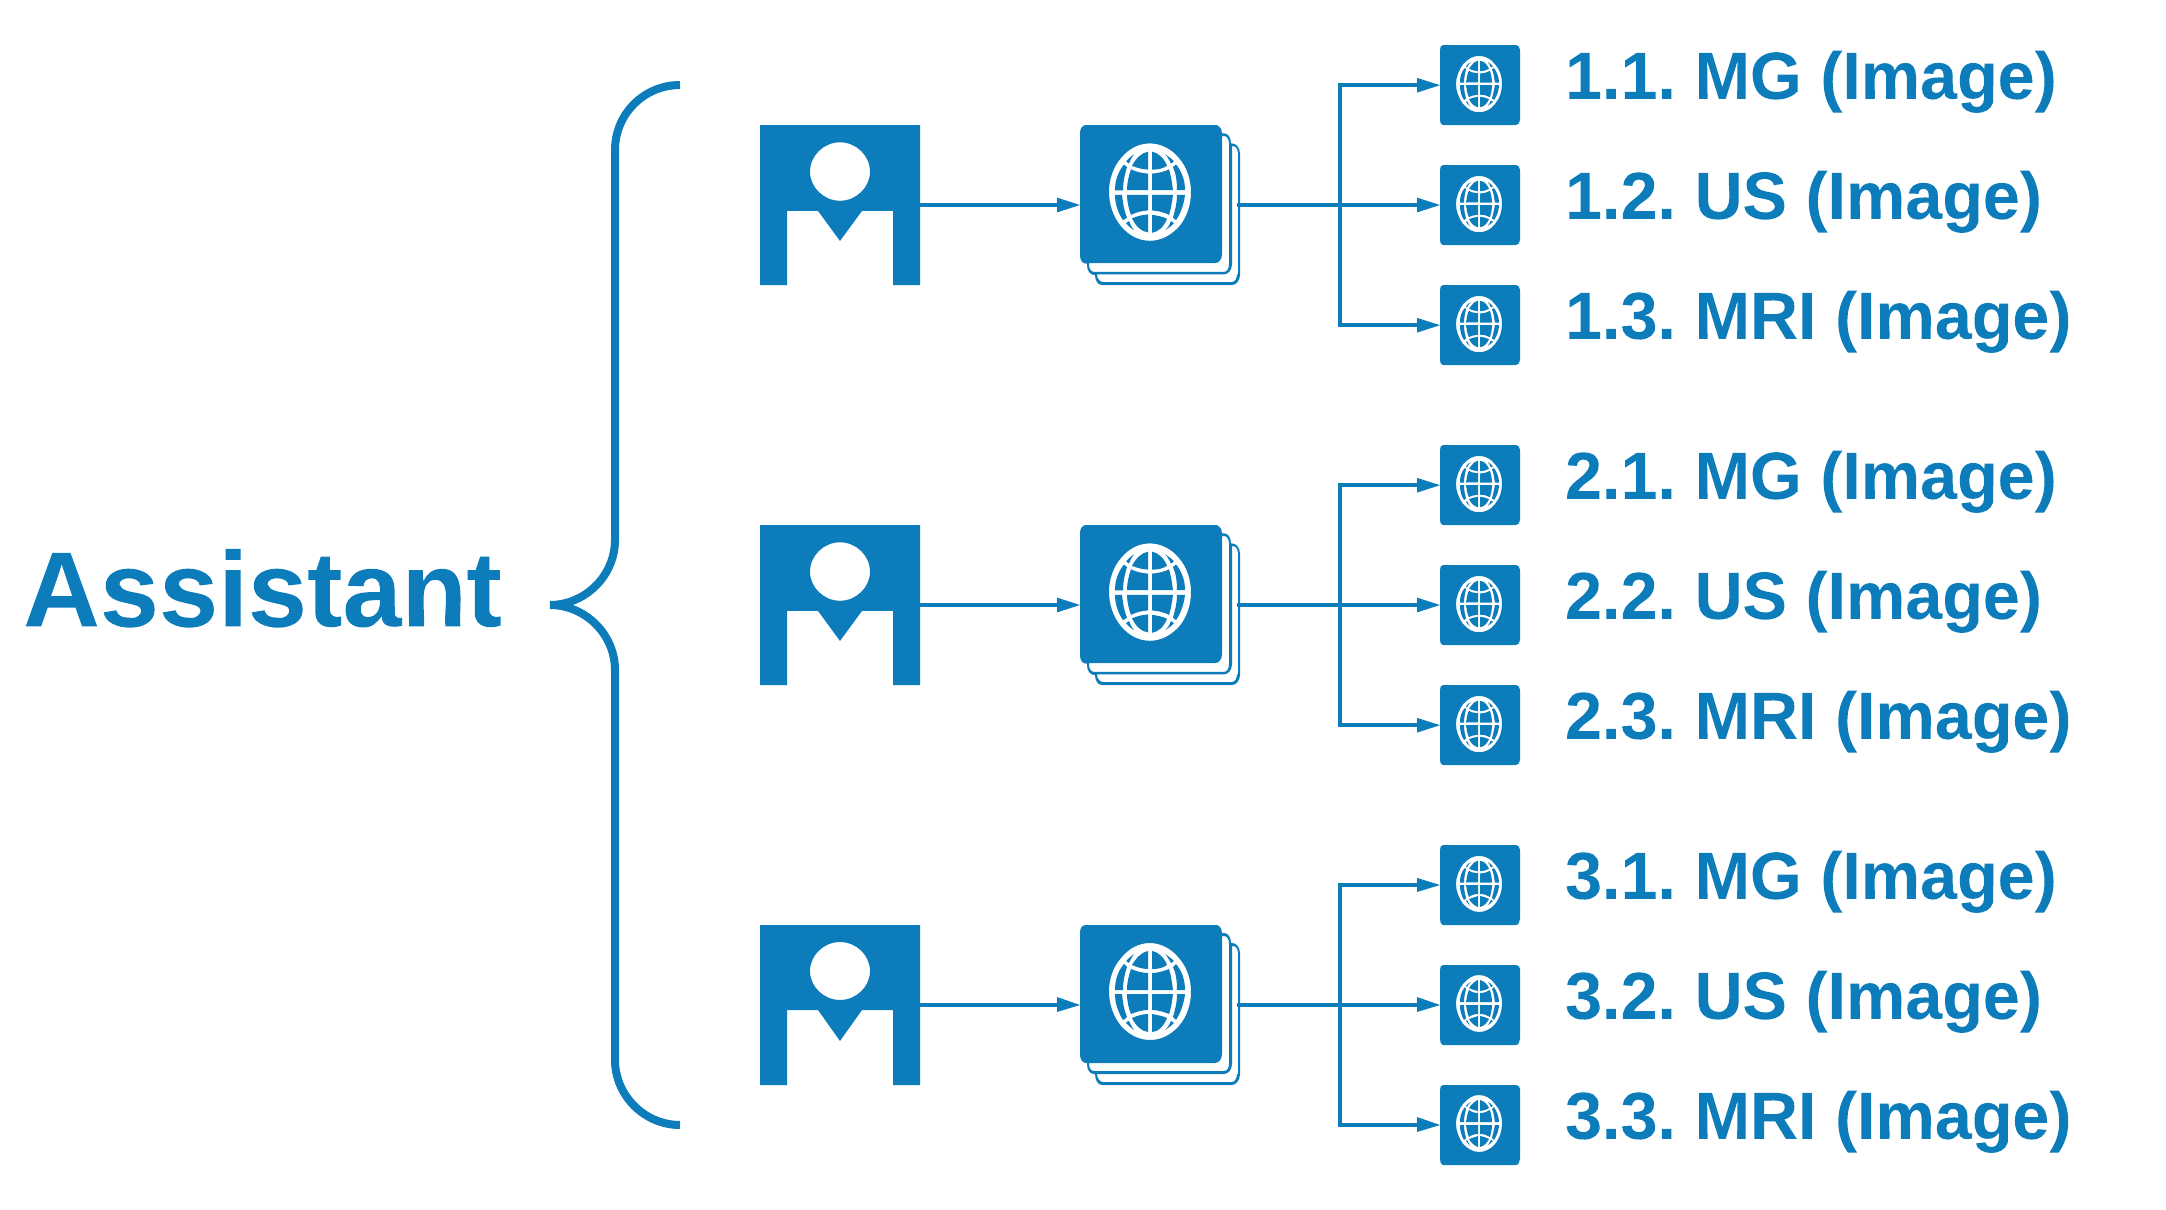
\includegraphics[width=0.50\textwidth]{img001}
\caption{Diagram representing the use of the \textbf{Assistant} by clinicians.}
\label{fig:svmm}
\end{wrapfigure}

\hfill

%%%%%%%%%%%%%%%%%%%%%%%%%%%%%%%%%%%%%%%%%%%%%%%%%%%

We will try to understand if, with the \textit{AI-Assisted} techniques, the clinicians will encounters the most accurate severity (\hyperlink{https://en.wikipedia.org/wiki/BI-RADS}{BIRADS}) of the breast lesions~\cite{american1998breast} and patient's prognostic. For this purpose, we have three patients (Figure \ref{fig:svmm}); each patient has three images in the respective modalities: (i) MG; (ii) US; and (iii) MRI. The clinicians will proceed to the activity of diagnosing the three patients within the support of our \textbf{Assistant} by the observation of ALL images.

\hfill

In our \textbf{User Testing Guide} a set of tasks is necessary and carefully crafted. Our test studies involve asking participants to perform a set of tasks. By looking at what our user need to do with our system, our tasks are realistic as possible. We are not describing the exact steps participants need to take. We achieve that by avoiding the precise language used as labels in our system. The tasks are emotionally neutrals. And we did several \hyperlink{https://www.nngroup.com/articles/pilot-testing/}{pilot tests} to prevent misleading situations saving us from wasting resources by accidentally use a lousy task or from getting bad data. The tasks are as follows.

\hfill

%%%%%%%%%%%%%%%%%%%%%%%%%%%%%%%%%%%%%%%%%%%%%%%%%%%

List of stand alone tasks:

%%%%%%%%%%%%%%%%%%%%%%%%%%%%%%%%%%%%%%%%%%%%%%%%%%%

\hfill

\begin{itemize}
\item[] \textbf{Task 1.1:} Classify \textit{Patient 1} on the \textbf{Assistant};
\item[] \textbf{Task 1.2:} Classify \textit{Patient 2} on the \textbf{Assistant};
\item[] \textbf{Task 1.3:} Classify \textit{Patient 3} on the \textbf{Assistant};
\end{itemize}

\hfill

\begin{itemize}
\item[] \textbf{Task 2.1:} Freely explore \textit{Patient 1} on the \textbf{Assistant};
\item[] \textbf{Task 2.2:} Freely explore \textit{Patient 2} on the \textbf{Assistant};
\item[] \textbf{Task 2.3:} Freely explore \textit{Patient 3} on the \textbf{Assistant};
\end{itemize}

\hfill

%%%%%%%%%%%%%%%%%%%%%%%%%%%%%%%%%%%%%%%%%%%%%%%%%%%

\clearpage
\section{Measurements}
\label{sec:sec007}

Our measurements refers to user performance measured against specific performance goals necessary to satisfy requirements. \textit{Task} completion success rates, adherence to dialog scripts, error rates and subjective evaluations will be used. \textit{Time-to-Completion} (TtC) of \textit{tasks} will also be collected. The measures are as follows.

\hfill

%%%%%%%%%%%%%%%%%%%%%%%%%%%%%%%%%%%%%%%%%%%%%%%%%%%

The tests are intended to achieve the following measures:

%%%%%%%%%%%%%%%%%%%%%%%%%%%%%%%%%%%%%%%%%%%%%%%%%%%

\hfill

\begin{itemize}
\item BIRADS Classification;
\item Pathology Classification;
\item Time measurement;
\item Number of clicks;
\item Number of errors;
\item Efficiency;
\item Difficulty;
\item Experience;
\end{itemize}

\hfill

%%%%%%%%%%%%%%%%%%%%%%%%%%%%%%%%%%%%%%%%%%%%%%%%%%%

To prioritise recommendations, a method for problem difficulty and degree severity classification, as well as, pathology importance, will be used in the analysis of the collected data during evaluation process. The approach treats problem severity has a combination of several factors. Those factors are measuring the impact of the problem and the frequency of users experiencing issues during the evaluation. Nevertheless, the opinion will also be of chief importance and we will also register the received ones.

\hfill

%%%%%%%%%%%%%%%%%%%%%%%%%%%%%%%%%%%%%%%%%%%%%%%%%%%

Through the questionnaire after the test session, we intend to obtain the answers to the following questions for each \textit{task}:

%%%%%%%%%%%%%%%%%%%%%%%%%%%%%%%%%%%%%%%%%%%%%%%%%%%

\hfill

\begin{itemize}
\item Acceptability of the \textbf{Assistant} lesion classification;
\item Acceptability of the \textbf{Assistant} interaction;
\item Acceptability of the \textbf{Assistant} translation;
\item Acceptability of the \textbf{Assistant} available features;
\item \textbf{Assistant} degrees of classification;
\item \textbf{Assistant} degrees of interaction;
\item \textbf{Assistant} degrees of information visualisation;
\end{itemize}

\hfill

%%%%%%%%%%%%%%%%%%%%%%%%%%%%%%%%%%%%%%%%%%%%%%%%%%%
\section{Goals}
\label{sec:sec008}

The next sections will describe the goals for \hyperlink{https://github.com/mida-project/prototype-multi-modality-assistant}{prototype-multi-modality-assistant} expectations. We will try to assess performance-related metrics such as time and correctness of participants completing \textit{tasks} for our expectations. Our expectations are based of the \hyperlink{https://docs.google.com/spreadsheets/d/1WwbvDO5Iz39Jr6H2ZzPth1o9DqhmpQz10Vtao7rvjfQ/edit?usp=sharing}{results} obtained at the lab as \hyperlink{https://www.nngroup.com/articles/pilot-testing/}{pilot tests}.

%%%%%%%%%%%%%%%%%%%%%%%%%%%%%%%%%%%%%%%%%%%%%%%%%%%
%                                                 %
%                     SECTION                     %
%                                                 %
%%%%%%%%%%%%%%%%%%%%%%%%%%%%%%%%%%%%%%%%%%%%%%%%%%%

\subsection{Completion Rate}

\textbf{Completion Rate} is the percentage of test participants who successfully complete the task without critical errors. A critical error is defined as an error that results in an incorrect or incomplete outcome. In other words, the completion rate represents the percentage of participants who, when they are finished with the specified task, have an "output" that is correct.

%%%%%%%%%%%%%%%%%%%%%%%%%%%%%%%%%%%%%%%%%%%%%%%%%%%

\hfill

\textit{A \textbf{Completion Rate} of \textbf{90\%} is the goal for each task in this usability test.}

\hfill

%%%%%%%%%%%%%%%%%%%%%%%%%%%%%%%%%%%%%%%%%%%%%%%%%%%

%%%%%%%%%%%%%%%%%%%%%%%%%%%%%%%%%%%%%%%%%%%%%%%%%%%

\hfill

\textbf{Note:} If a participant requires assistance in order to achieve a correct output then the task will be scored as a critical error and the overall completion rate for the task will be affected.

\hfill

%%%%%%%%%%%%%%%%%%%%%%%%%%%%%%%%%%%%%%%%%%%%%%%%%%%

%%%%%%%%%%%%%%%%%%%%%%%%%%%%%%%%%%%%%%%%%%%%%%%%%%%
%                                                 %
%                     SECTION                     %
%                                                 %
%%%%%%%%%%%%%%%%%%%%%%%%%%%%%%%%%%%%%%%%%%%%%%%%%%%

\subsection{Error-Free Rate}

\textbf{Error-Free Rate} is the percentage of test participants who complete the task without any errors (critical or non-critical errors). A non-critical error is an error that would not have an impact on the final output of the task but would result in the task being completed less efficiently.

%%%%%%%%%%%%%%%%%%%%%%%%%%%%%%%%%%%%%%%%%%%%%%%%%%%

\hfill

\textit{An \textbf{Error-Free Rate} of \textbf{80\%} is the goal for each task in this tests.}

\hfill

%%%%%%%%%%%%%%%%%%%%%%%%%%%%%%%%%%%%%%%%%%%%%%%%%%%

%%%%%%%%%%%%%%%%%%%%%%%%%%%%%%%%%%%%%%%%%%%%%%%%%%%
%                                                 %
%                     SECTION                     %
%                                                 %
%%%%%%%%%%%%%%%%%%%%%%%%%%%%%%%%%%%%%%%%%%%%%%%%%%%

\subsection{Time on Task (ToT)}

The time to complete a scenario is referred to as "Time on Task" (ToT). It is measured from the time the participant begins the scenario to the time which the participant signals completion.

%%%%%%%%%%%%%%%%%%%%%%%%%%%%%%%%%%%%%%%%%%%%%%%%%%%
%                                                 %
%                     SECTION                     %
%                                                 %
%%%%%%%%%%%%%%%%%%%%%%%%%%%%%%%%%%%%%%%%%%%%%%%%%%%

\subsection{Subjective Measures}

Subjective opinions about specific tasks, time to perform each task, features, and functionality will be surveyed. At the end of the test, participants will rate their satisfaction with the overall system. Combined with the interview/debriefing session, these data are used to assess attitudes of the participants.

%%%%%%%%%%%%%%%%%%%%%%%%%%%%%%%%%%%%%%%%%%%%%%%%%%%
\section{Reporting Results}
\label{sec:sec009}

A \hyperlink{https://github.com/mida-project/research-reports}{Test Report} will be provided at the end of this tests. It will consist of a report and/or a presentation of the results; evaluation of the metrics against the pre-approved goals, subjective evaluations, and specific issues of the system, as well as, recommendations for resolution. The recommendations will be categorically sized by development to aid in implementation strategy. The results will be translated to a \hyperlink{https://docs.google.com/spreadsheets/d/1CoPLONnINdBWryGs7SBRuPZA-DnQ0t_yzx3u8ym0UoI/edit?usp=sharing}{spreadsheet} (view only). Also, more related information can be found at \hyperlink{https://github.com/MIMBCD-UI/prototype-breast-screening/wiki/User-Test-Evaluation}{Test 4: Assistant}.

\clearpage

\bibliographystyle{plain}
\bibliography{bibliography/references.bib}

\end{document}